\PassOptionsToPackage{unicode}{hyperref}
\PassOptionsToPackage{naturalnames}{hyperref}
\documentclass[12pt, xetex, xcolor=pdftex, dvipsnames]{beamer}
\usetheme{metropolismyfont}
\usepackage{dcolumn} % for apsrtable outputs
\usepackage{xunicode} % extra support for unicode
\usepackage{xltxtra} % implements some odds-and-ends features
\usepackage{verbatim} % for multiple-line comments
% to fix a problem in line-breaks
% see "http://zrbabbler.hp.infoseek.co.jp/xelatex.html"
\XeTeXlinebreaklocale "ja"
\XeTeXlinebreakskip=0pt plus 1pt
\XeTeXlinebreakpenalty=0
\def\<{\@ifstar{\zx@hwback\nobreak}{\zx@hwback\relax}}
\def\zx@hwback#1{\leavevmode#1\hskip-.5em\relax}

\usepackage{color}
\usepackage{listings}
\lstset{%
    language={Python},%
    basicstyle={\footnotesize},%
    identifierstyle={\footnotesize},%
    commentstyle={\footnotesize\color{mLightGreen}},%
    keywordstyle={\footnotesize\color{mLightBrown}},%
    stringstyle={\footnotesize\color{mDarkBrown}},%
    frame={tblr}%
}

\usepackage{graphicx}

\AtBeginSection[]{
    \begin{frame}{目次}
        \setbeamertemplate{section in toc}[sections numbered]
        \tableofcontents[currentsection, hideallsubsections]
    \end{frame}
}

\title{引き継ぎ資料 Vol.4}
\subtitle{オブジェクトの話}
\date{2016/08/??}
\author{}
\institute{}
\begin{document}
\maketitle
\begin{frame}{コンセプト}
    ``オブジェクトって何?''を解決
\end{frame}
\begin{frame}{目次}
  \setbeamertemplate{section in toc}[sections numbered]
  \tableofcontents[hideallsubsections]
\end{frame}

\section{導入}
\begin{frame}{導入}
    \begin{block}{Q.}
        {\Large オブジェクトって何?}
    \end{block}
    \pause
    \begin{alertblock}{A.}
        データや構造としての{\Large ``何か''}
    \end{alertblock}
\end{frame}
\begin{frame}[fragile]{例}
\begin{lstlisting}
>>> int_variable = 10  # int object
>>> flaot_variable = 3.7  # float object
>>> str_object = "Hello"  # str object
>>> none_object = None  # NoneType object
>>> list_object = []  # list object
>>> dict_object = {}  # dict object

>>> # numpy.ndarray object
>>> array_object = numpy.array([1, 2, 3])
\end{lstlisting}
\pause
なんでもオブジェクト
\end{frame}
\begin{frame}{オブジェクトの中身}
\begin{itemize}
    \item 関数(正確にはメソッド)
    \item 他のオブジェクト
\end{itemize}
\end{frame}
\begin{frame}[fragile]{例}
\begin{lstlisting}
>>> list_object = [1, 2, 3, 4]  # list object
>>> # list_objectの中にあるappendメソッド
>>> list_object.append(5)
>>> # list_objectがappendという操作を受け付けて
>>> # リストの中に5を追加
>>> print(list_object)
[1, 2, 3, 4, 5]
>>> # numpy.ndarray object
>>> array_object = numpy.array([
...     [1, 2, 3],[4, 5, 6]
... ])
>>> print(a.shape)  # aの中のタプルオブジェクト
(2, 3)
\end{lstlisting}
\end{frame}
\begin{frame}{型}
    オブジェクトは様々な中身を持つことが可能

    中身のテンプレート$\rightarrow$型
\end{frame}
{
    \setbeamertemplate{frame footer}{%
        Photo credit: \href{https://www.flickr.com/photos/bittermelon/3293430756/}{bittermelon} %
        via \href{http://foter.com/}{Foter.com} %
        / \href{http://creativecommons.org/licenses/by-nc/2.0/}{CC BY-NC}%
    }
    \usebackgroundtemplate{\includegraphics[width=\paperwidth]{img/taiyaki.jpg}}
    \begin{frame}{オブジェクトの作成=型から物を作成}
    \end{frame}
}
\begin{frame}
    型って自分で作れないの?

    \pause
    自作できる型$\rightarrow$クラス
\end{frame}

\section{クラス}
\begin{frame}{クラスの話をする前に\dots}
    Cの{\Large ``構造体''}覚えてますか?
\end{frame}
\begin{frame}{クラス}
    クラス\dots Cの構造体{\Huge\alert{$+\alpha$}}

    \pause
    $+\alpha$の部分がとても巨大
\end{frame}
\begin{frame}[fragile]{復習 -- 構造体 --}
    ``車''を表す構造体

    \lstinputlisting[language=C, firstline=3, lastline=6]{../src/struct.c}

    \begin{itemize}
        \item メンバはxとy
        \item それぞれには.でアクセス
    \end{itemize}
\end{frame}
\begin{frame}[fragile]{復習 -- 構造体 --}
    \lstinputlisting[language=C, firstline=12]{../src/struct.c}

    car1とcar2は別物

    \pause
    car1とcar2はCar型のオブジェクト
\end{frame}
\begin{frame}[fragile]{Pythonで構造体的なこと}
    \lstinputlisting[firstline=1, lastline=11]{../src/class_sample.py}
    Carはクラス
\end{frame}
\begin{frame}{\_\_init\_\_}
    \lstinputlisting[firstline=1, lastline=4]{../src/class_sample.py}

    \begin{itemize}
        \item \_\_init\_\_は関数
        \item クラスの中に宣言されている$\rightarrow$メンバ関数
        \item オブジェクトの作成時に呼び出し
        \item selfは自分自身を指す
    \end{itemize}
\end{frame}
\begin{frame}[fragile]{2つのrun関数は同じ処理}
    \lstinputlisting[firstline=1, lastline=13]{../src/class_self.py}
\end{frame}
\begin{frame}{メンバ関数}
    どちらの関数でも同じ処理が可能

    \pause メンバ関数が不要?

    \pause \alert{そんなことはない}
\end{frame}
\begin{frame}[fragile]{2つのrun関数は同じ?}
    \lstinputlisting[firstline=1, lastline=8]{../src/class_require.py}
    \begin{itemize}
        \item 関係あるものは関係する場所に配置
        \item 事故防止は大事
    \end{itemize}
    \pause
    \alert{メンバ関数超大事}
\end{frame}
\begin{frame}{オブジェクト指向}
    プログラム全体をオブジェクトの集合で構成する手法

    \begin{exampleblock}{概念}
        \begin{itemize}
            \item カプセル化
            \item 継承
            \item ポリモーフィズム
        \end{itemize}
    \end{exampleblock}
\end{frame}

\section{カプセル化}
{
    \setbeamertemplate{frame footer}{%
        Photo credit: \href{https://www.flickr.com/photos/aidanmorgan/4634923304/}{John-Morgan} %
        via \href{http://foter.com/}{Foter.com} %
        / \href{http://creativecommons.org/licenses/by/2.0/}{CC BY}%
    }
    \usebackgroundtemplate{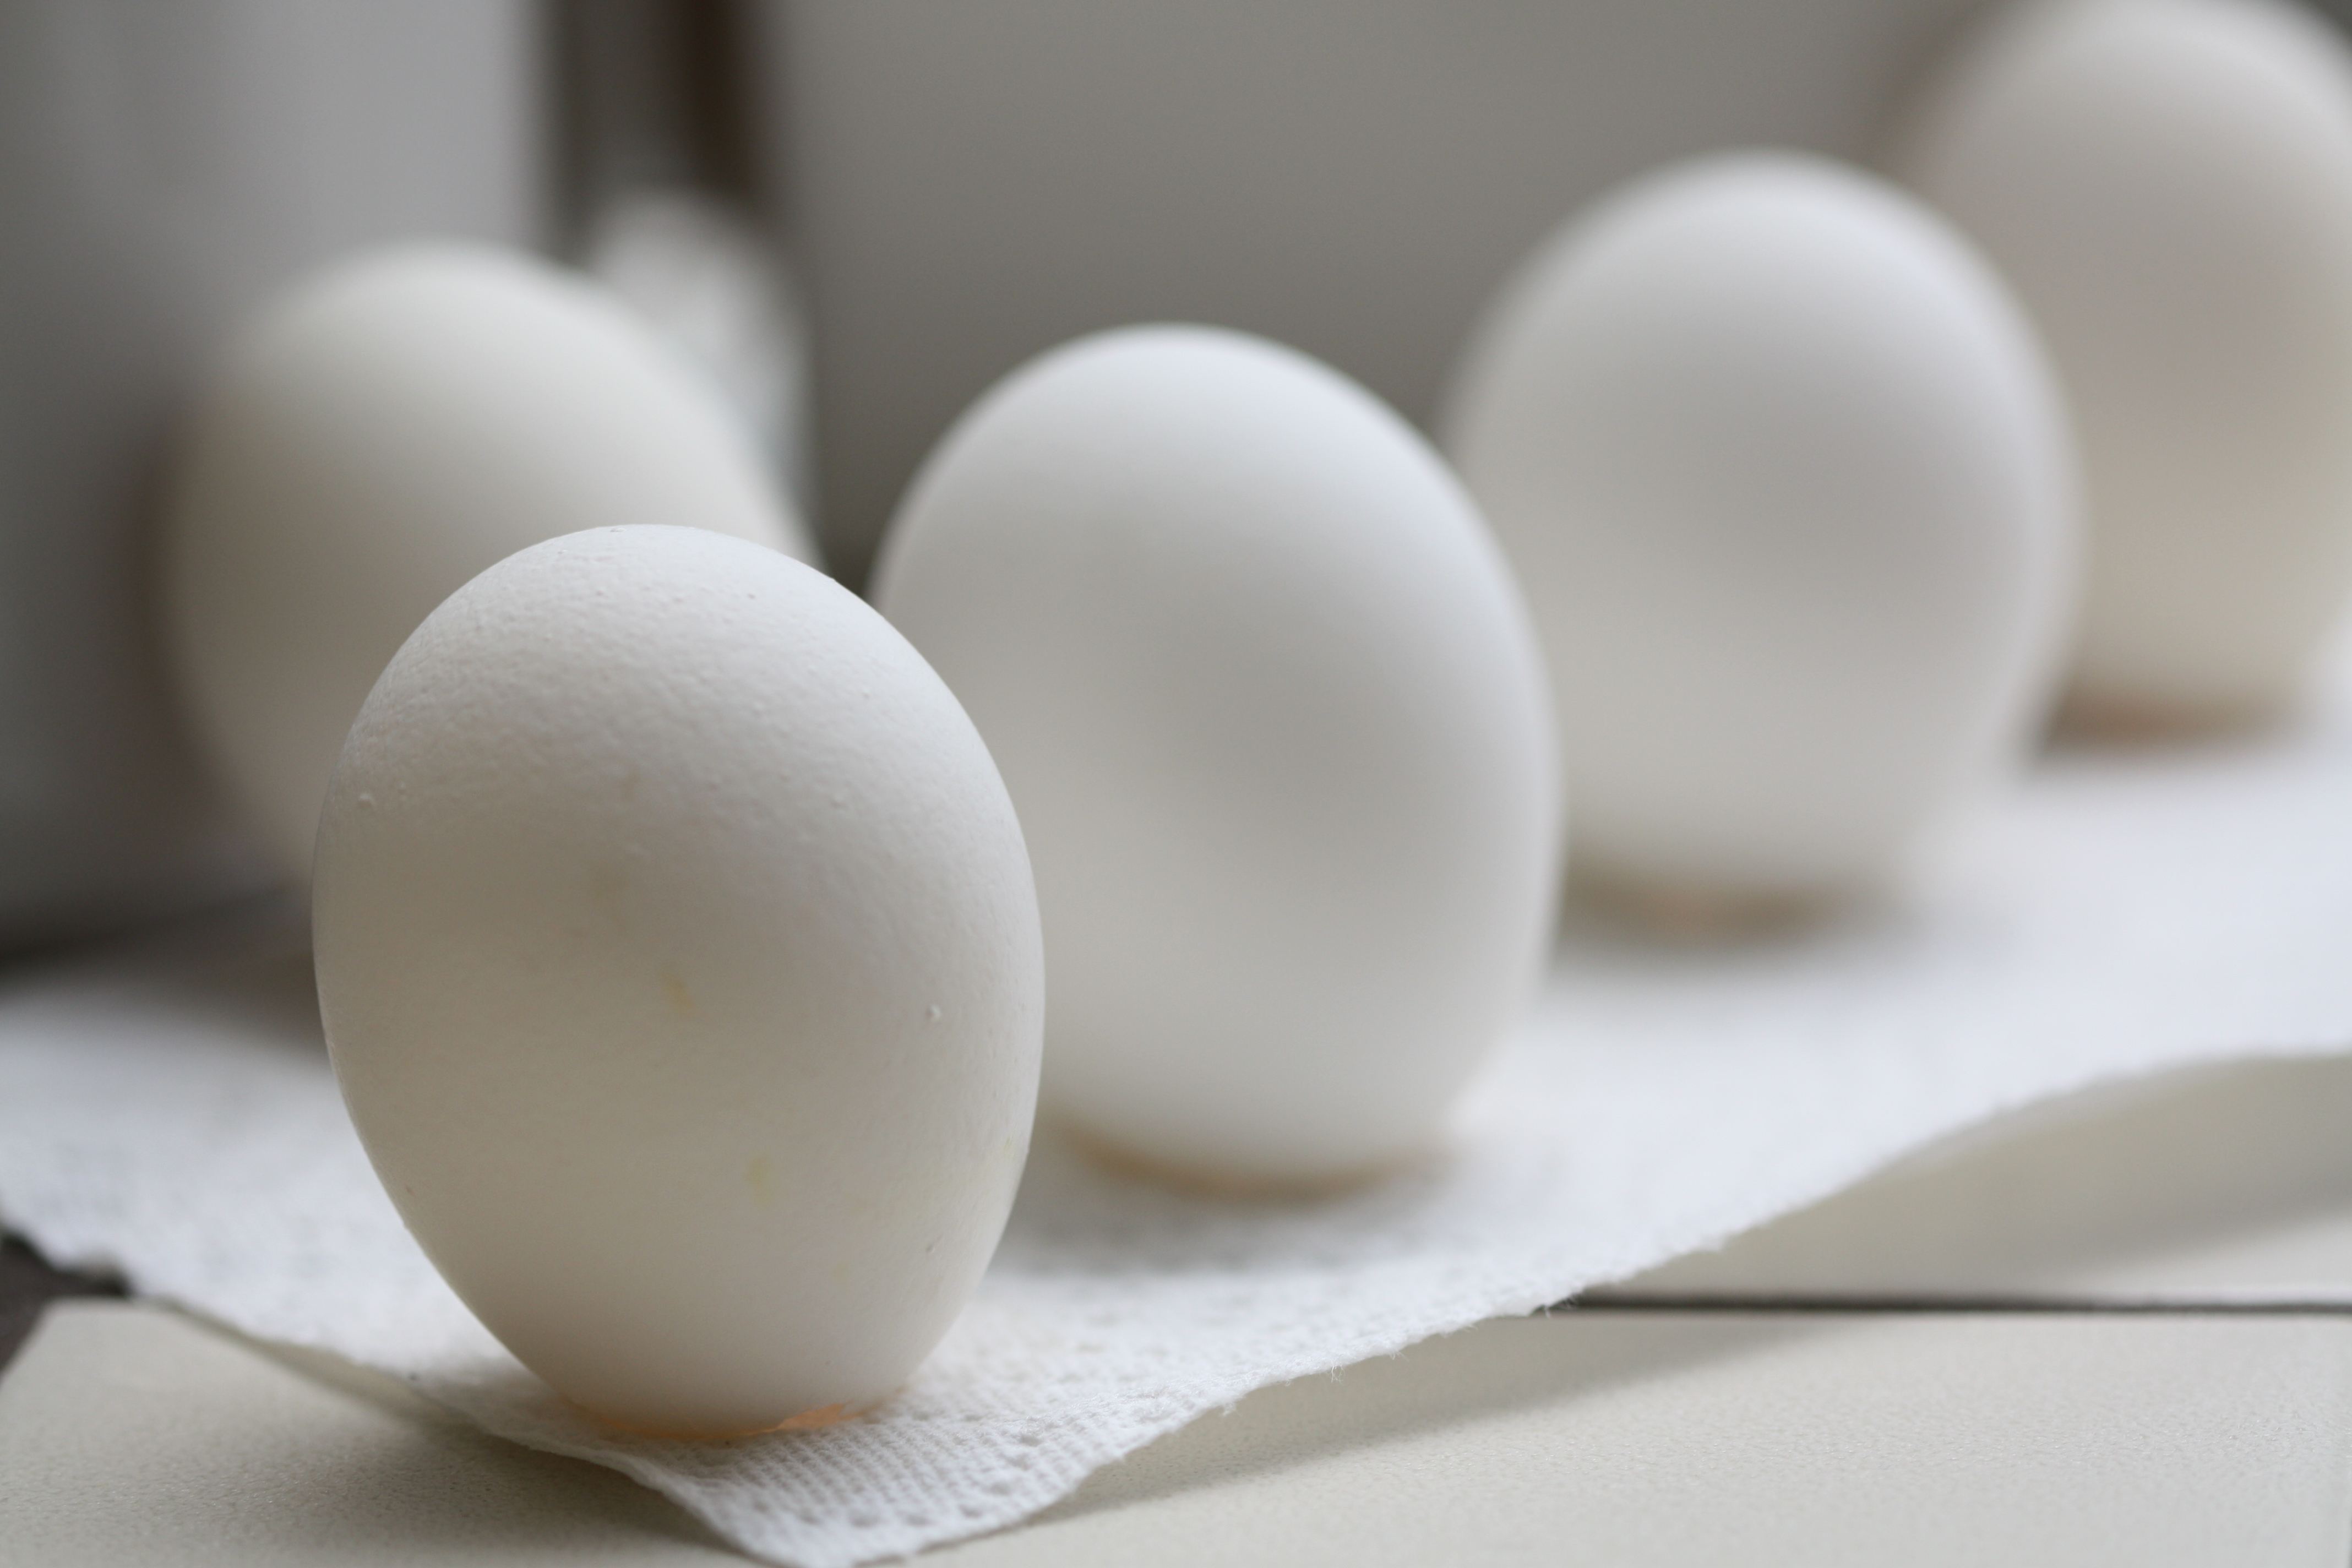
\includegraphics[width=\paperwidth]{img/egg.jpg}}
    \begin{frame}{カプセル化 = クラスの中身を隠蔽}
    \end{frame}
}
\begin{frame}[fragile]{例}
    Carクラスに燃料の概念を追加
    \lstinputlisting[lastline=7]{../src/no_encapsulation.py}

    \pause
    \begin{block}{問題点}
        車内部のガソリン(gas)を外部から操作可能
    \end{block}
\end{frame}
\begin{frame}{問題点なのか?}
    この状態なら燃料を操作されて困ることは無い\onslide<2->{{\Huge が}}

    \onslide<3->
    例えばこれが
    \begin{itemize}
        \item 重要なフラグ
        \item 変更された時に何らかの処理をしたい変数
    \end{itemize}
    だったなら?
\end{frame}
\begin{frame}[fragile]{例}
    \lstinputlisting[lastline=7]{../src/no_encapsulation_meter.py}
    どうやってlamp関数を呼び出すか?
\end{frame}
\begin{frame}[fragile]{解}
    \lstinputlisting[firstline=9, lastline=14]{../src/no_encapsulation_meter.py}
    \pause
    \begin{block}{問題点}
        Carを使う側がlampを知っている必要あり

        \alert{自動でランプは起動しない!}
    \end{block}
\end{frame}
\begin{frame}[fragile]{カプセル化を使用}
    \lstinputlisting[lastline=13]{../src/encapsulation_meter.py}
\end{frame}
\begin{frame}{カプセル化を使用}
    \begin{itemize}
        \item Carを使う側はlampを知らなくていい
        \item gasに応じた処理を内部に追加可能
        \begin{itemize}
            \item 追加されてもユーザは知らなくていい
        \end{itemize}
    \end{itemize}
\end{frame}
\begin{frame}{カプセル化}
    \begin{itemize}
        \item 外部から見えていいもの・いけないものを区別
        \item アクセス権限を制御
    \end{itemize}
    \begin{table}
        \centering
        \caption{アクセス権限}
        \begin{tabular}{lll}
            \hline
            名称 & 範囲 & 命名規則\footnotemark \\\hline
            private & 自分のクラス内 & \_\_から名前を開始 \\\hline
            protected & 自分と継承先内 & \_から名前を開始 \\\hline
            public & どこからでも & \_をつけない \\\hline
        \end{tabular}
    \end{table}
    \footnotetext{\href{https://google.github.io/styleguide/pyguide.html}{Google Python Style Guide}}
\end{frame}
\begin{frame}{注意点}
    \begin{itemize}
        \item Pythonはprivateでも外から呼ぶことが可能
        \item privateなものを外から呼んではいけない\\
            \alert{private = 外から呼ぶなという意思表示}
        \item \_から始まるものは外から呼ばない!
    \end{itemize}
\end{frame}
\begin{frame}{まとめると...}
    ゲームの中身を知らなくても遊べるでしょうって話

    改造してはいけない
    \begin{figure}
        \centering
        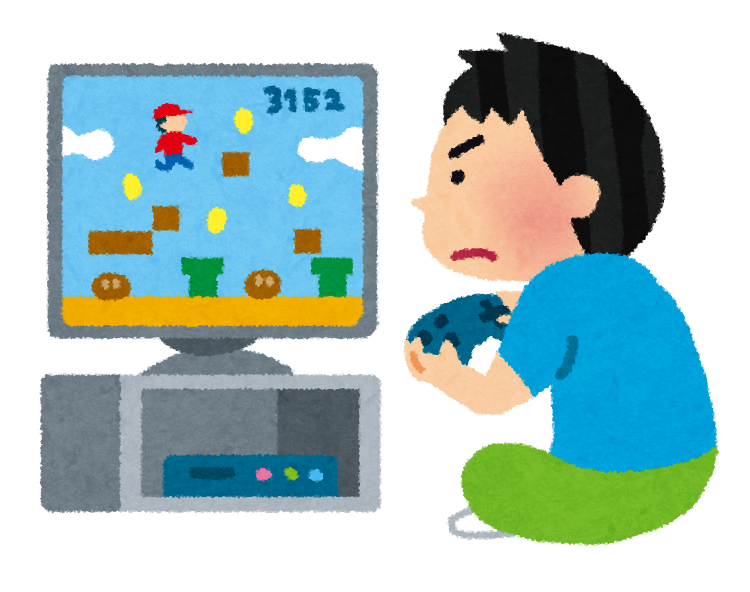
\includegraphics[width=7cm]{./img/videogame_boy.png}
    \end{figure}
\end{frame}

\section{継承}

\section{ポリモーフィズム}

\section{まとめ}
\begin{frame}
    ``オブジェクト''の概念は使いこなせば便利

    データ解析の分野では作る必要は無い可能性が高い

    使えないのは危険
\end{frame}
\begin{frame}[standout]
  Questions?
\end{frame}
\end{document}
